\section{Introduction}
\label{sec:introduction}

% state the learning objective 
The objective of this laboratory assignment is to choose the dimensions and implement a BandPass Filter (BPF) with the a central frequency of 1kHz and a gain of 40dB (at central frequency). \par
The components used:\par
- One 741 OPAMP; \par
– At most three 1k$\Omega$ resistors; \par
– At most three 10k$\Omega$  resistors; \par
– At most three 100k$\Omega$  resistors; \par
– At most three 220nF capacitors;\par
– At most three 1$\mu$ F capacitors; \par

Firstly, we started this laboratory writing an NGspice script that simulates the bandpass filter (BPF), based on the script given, using the provided OPAMP model. This simulation is design to measure the output voltage gain in the passband, the central frequency and the input and output impedances at this frequency. \par
Then, we have performed incremental modifications to improve the merit, which is calculated using the expression: \par
\begin{equation}
    M = \frac{1}{Cost \times (gain_{deviation} + CentralFrequency_{deviation} + 10^{-6})}
\end{equation}\par
Where:\par
- cost = cost of resistors + cost of capacitors + cost of transistors; \par
– cost of resistors = 1 monetary unit (MU) per kOhm; \par
– cost of capacitors = 1 MU/$\mu$ F; \par
– cost of transistors = 0.1 MU per transistor; \par

After that, using octave, we have created a theoretical analysis able to compute the gain, input and output impedances at the central frequency. \par
The, we have also computed the frequency response $V_{o}(f)/V_i{f}$, using the incremental analysis, solving the circuit for a frequency vector in log scale with 10 points per decade, from 10Hz to 100MHz.\par

Firstly, we have created a simple circuit and then we were updating the circuit to improve the figure of merit. The final circuit obtainned is the one shown below in figure (Fig.\ref{fig:circuito}): \par

\begin{figure}[H]
\centering
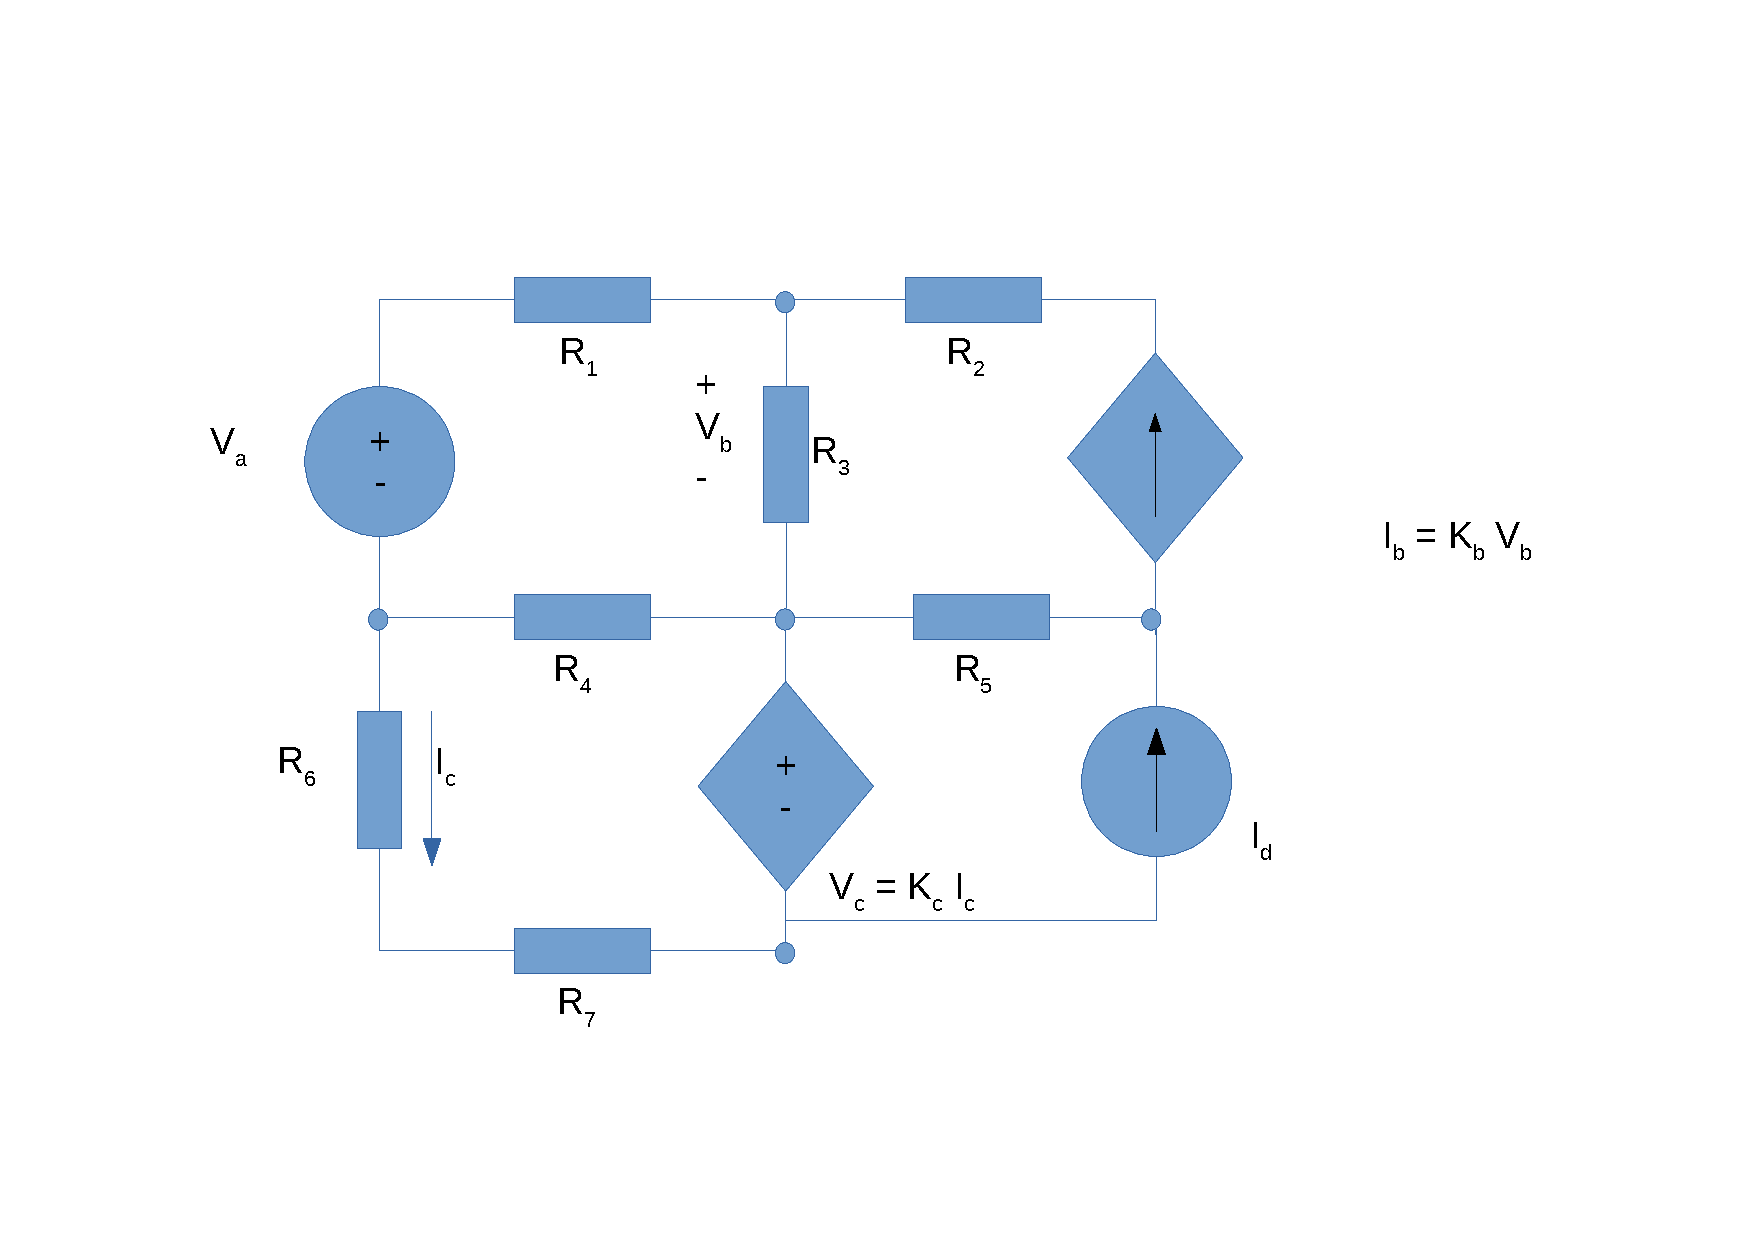
\includegraphics[width=0.9\linewidth]{circuito}
\caption{Final circuit}
\label{fig:circuito}
\end{figure}

The individual costs of the components used: 

\begin{center}
  \begin{tabular}{ | c | c | }
    \hline    
    {\bf Name} & {\bf Value} \\ \hline
    $R$ & 103k$\Omega$ \\ \hline 
    $C$ & 0.330 $\mu$S \\ 
    \hline
  \end{tabular}
  \captionof{figure}{Costs}
\end{center}



